\setchapterpreamble[u]{%
	\dictum[Christiane Taubira refiriéndose al presidente Macron.]{Los fracasos políticos son temporales, pero las derrotas semánticas y
	culturales son dramáticas porque tardan más en revertirse.}
	}
\chapter{Lee esto antes de \emph{hacer} algo}
\label{cha:antesalgo}

El nuestro es un mundo de redes, navegable a través de teorías de la complejidad y del caos. Muchos procesos automáticos alimentan diariamente el flujo de operaciones de las infraestructuras (redes de abasto de combustibles, electricidad para servidores, satélites, líneas de internet) sin que haya realmente un responsable. Las funciones están programadas y los destinos predeterminados. Miles de variables interactuando entre ellas a partir de distintos nodos que envían información diversa y que demandan u ofertan certificados, \emph{requests}. La idea de la cibernética es dispersar para crear un caos gestionable, incluso automatizable.

\begin{figure}[htbp]
	\centering
	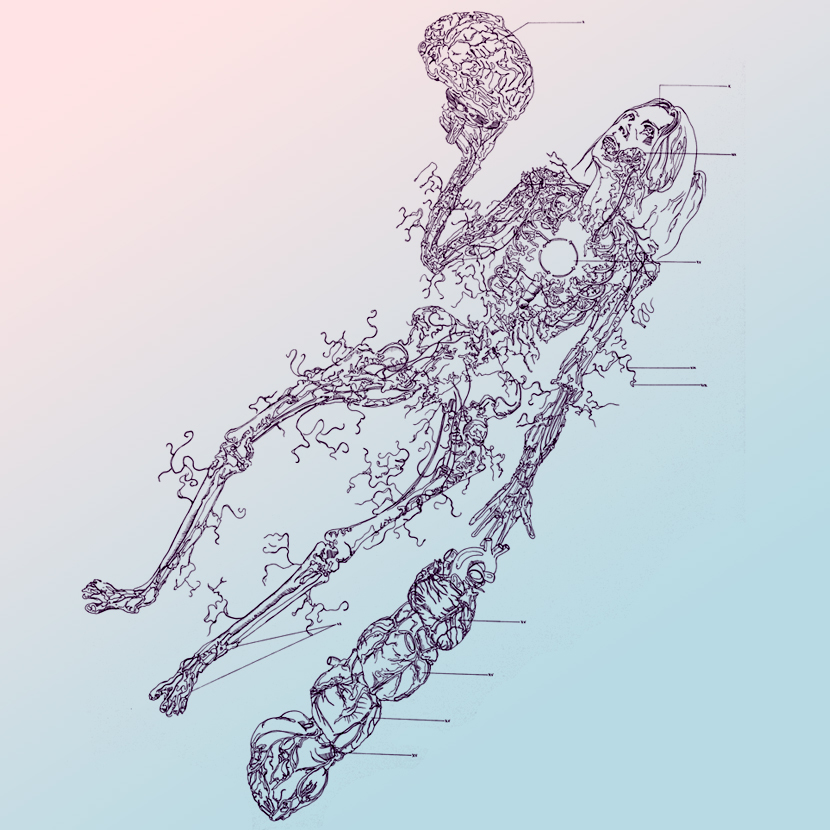
\includegraphics[width=\linewidth]{zombie.jpg}
	\caption{¿Cyborg o zombi?}
	\label{fig:cyberzombie}
\end{figure}

Al mismo tiempo tenemos lo necesario para implementar una economía \hlfix{posescasez}{Me parece que es más correcto escribir \emph{postescasez}.},\footnote{\url{es.wikipedia.org/wiki/Economía\_post-escasez}} sólo se trata de intervenir estratégicamente en esas redes de información, que también son flujos de sentido, producciones de deseo. La utopía robótica es una de las aristas de distintos escenarios posibles planteados por el texto de Peter Frese titulado \emph{Four Futures}, donde señala que viviremos en un mundo materialmente condicionado por dos aristas, una de igualitarismo-estamentalismo (o sea, donde las jerarquías manden) y otra de abundancia (por la automatización tecnológica) o escasez (por nuevas formas de los patrones para crear valor explotable). De esos casos, los más extremos parecen ser el mundo donde quepan todos los mundos, sostenido por una infraestructura tecnológica común, y el exterminio, que es prácticamente lo mismo pero solo para 1~\% de la población global.\footnote{A ello habría que sumar el problema del deseo, pensar en los desarrollos cibernéticos de las economías libidinales o economías del deseo.}

\begin{table}
	\caption{}
	\todo[inline]{Añadir una leyenda a la tabla. Se hizo flotante para poder asignarle una referencia cruzada y vincularla a la sección~\ref{sec:viruscapitalista}, donde se le cita.}
	\label{tab:Aristas}
	\centering

	\begin{tabular}{lll}
		\toprule
		 & \textbf{Abundancia} & \textbf{Escasez}\\
		\midrule
		\textbf{Igualdad} & Comunismo & Socialismo\\
		\textbf{Jerarquía} & Rentismo & Exterminismo\\
		\bottomrule
	\end{tabular}
\end{table}

Según Natalie Wynn\footnote{Famosa por ContraPoints, su vlog en YouTube.}, la derecha de internet pinta una caricatura de la izquierda, con el marxismo posmoderno como la supuesta ideología. Esto es muestra de que una de las operaciones más efectivas del parásito capitalista es poner a pelear a las resistencias en torno a cosas pequeñas y concretas,\footnote{Freud se refiere a esto como el narcisismo de las pequeñas diferencias.} cuando es más aquello en lo que estamos de acuerdo pero tenemos la necesidad de encontrar coherencia teórica en modelos ideales y no en especulaciones sobre la realidad. Esta posición que renuncia a la necesidad de certidumbre intelectual ---es decir, que no va más allá de una pregunta sobre instancias, sobre cómos--- se conoce como realismo especulativo y es cercana a una teoría del conocimiento (y filosofía del ser) llamada \enquote{ontología orientada a objetos}.\revquotes{} Es importante recordar que probablemente las civilizaciones humanas han sido injustas desde el principio de los tiempos, pero la posición que tomamos respecto a la explotación de los patrones, de los propietarios o de los banqueros depende en buena medida de dónde estamos paradas.

Como reza el lema del xenofeminismo:
	
\begin{quote}
	\textsf{\textbf{Si la naturaleza es injusta, ¡cambiémosla!}}
\end{quote}

Podemos hablar desde el arte, generando consensos en torno a acciones comunes en distintos grupos. A veces parece más fácil actuar desde los medios que desde la militancia de izquierda. Nuestras aliadas han repetido ya varias veces la necesidad de hacer un posicionamiento estético sobre el discurso. En nuestros tiempos, en la política rige el principio de que fondo es forma. Y sin embargo, son las cuestiones estructurales como el género, el color de piel, la nacionalidad, el acceso a educación, salud, el dinero, etc, las que más afectan, por una cuestión de origen, de diseño, sobre las tecnologías que configuran nuestra realidad.

Al ser un concepto y no el nombre de un objeto concreto, la influencia del capitalismo se toma por la derecha como un mero principio económico que brinda todas las mercancías necesarias para vivir cómodo. He aquí una de las partes más importantes del problema. Para entenderlo, tenemos que comprender las diferencias entre Estado y Capitalismo en la historia, y cómo funciona a grandes rasgos el espectro político a partir de estas diferencias. Sin embargo, el pensamiento del \emph{status quo} es realmente poderoso pues el Estado dispone de manera muy particular de las armas que reproducen el modo de producción capitalista, las orienta siempre a la eficiencia y optimización que produce valor intercambiable.

\section{¿El enemigo es el capitalismo, el Estado o los mercados?}
\label{sec:enemigos}

Ahora vamos a profundizar en algunas distinciones que sirvan para hacer cosas que generen cambios reales. Sabemos que en este análisis hemos hablado poco del patriarcado pues lo asumimos como parte de la ideología primigenea del capitalismo. Ponga usted mucha atención porque ahí vamos:

El capitalismo, desde una \emph{visión de ingeniero},\didit{se resaltó el término} se trata básicamente de un modo de producción de bienes materiales. Este modo de hacer cosas parte de factores de producción que tradicionalmente han sido resumidos como tierra, capital y trabajo. El marxismo fue importante porque nos mostró un análisis mucho más extenso del capitalismo, al entenderlo como una configuración de las relaciones sociales a través de los procesos productivos, donde las mercancías tienen un valor por sí mismo y tan poderoso que configuran la identidad misma de las subjetividades.

Para nosotras, además de lo que le aprendimos al marxismo clásico, el capitalismo es un modo de producción pero en este momento de la historia también es una \emph{velocidad sobre los flujos de información}. Para sostener lo anterior, es necesario que comprendamos que el viejo escenario económico donde la fábrica jugaba el rol predominante en la producción de valor ha sido reemplazado por una lógica de trabajo que pulveriza y divide en diferentes espacios la línea de producción, de manera que sea más eficiente y barato producir. Y lo que genera más valor en la economía contemporánea no es ya la mercancía como un objeto físico sino la información que producen las relaciones entre las cosas. A esta era de la economía algunas personas la llaman \emph{posfordismo}\todo{Sugiero cambiar por \emph{postfordismo}.} y entre otras cosas, es más una forma de producción regida por el consumo, es decir, la demanda de bienes, que por la producción, como lo fue en las revoluciones tecnológicas pasadas.

El mercado es un conjunto de transacciones. Es la infraestructura del intercambio mercantil y su acontecer capitalista tiene más que ver más con el cobro del impuesto, origen de la financiarización del valor,\footnote{Garzon Espinosa, Alberto. \enquote{¿Qué es la financiarización?} en \emph{Economía Crítica y Crítica de la Economía}. Disponible en:~\url{www.economiacritica.net/?p=144}.} que con el comercio. El capitalismo es un parásito cultural que paraliza el trabajo y subsume los recursos y hábitats del planeta mientras mercantiliza bienes primarios (\emph{raw materials}) en abstracciones virtuales, a través de una economía del deseo. Se in-corpora (es decir, configura una respuesta física, corporal) en las relaciones de las personas y crece sin límites hasta que mata al huésped. Además, es contagioso. Se ajusta a afectos y deseos de los huéspedes mientras que se adapta a esa lógica en particular. Su funcionamiento produce un ecosistema. Imagina que además de una configuración sobre las velocidades, el capitalismo es un parásito que infecta los grupos sociales, una suerte de falla en la naturaleza que nos impide relacionarnos directamente.\footnote{Para ello, recordemos que la experiencia humana es tan antinatural, tan cyborg, como una ciudad, como el internet o como la resina que implantan en tus dientes cuando tienes caries. Y que hablar de lo natural no implica de ninguna manera que algo sea justo. De ahí una frase que retoma el xenofeminismo: si la naturaleza es injusta, cambiémosla.} El propósito de este parásito es acumular cada vez más. La inteligencia del parásito reproduce la lógica de un virus informático. Es decir, hoy en día el capitalismo como parásito vivo es concretamente un algoritmo. Si la sociedad funciona como un sistema vivo, el capitalismo es el virus que infecta las relaciones sociales para convertirlas en relaciones mercantiles, con la única intención de mantenerse como necesario. En ese sentido, juega un rol parecido al Estado en la medida en que actúa como intermediario de toda relación social. Sin embargo, si el mercado es el medio del capital, \emph{el Estado es el soporte de información del mercado}, es el medio de almacenamiento y transmisión de la información del mercado que no puede ser retenida en la contabilidad. El Estado es una expresión de tecnologías del poder, con instancias materiales concretas. Más allá de la ideología, el poder se despliega a través de un conjunto de tecnologías.

El gobierno justifica la recaudación de impuestos al proveer servicios que hasta el momento consideramos que los mercados no podrán proveer (en buena medida por el control del capital). En términos de dinámicas de toma de decisión, el Estado es la masa personificada o \enquote{agenciada},\revquotes{} es decir, una entidad que puede trabajar como un agente. De ahí la necesidad de sistemas de recaudación en red que partan de una reconfiguración de las subjetividades y por tanto, de la comprensión de lo público, lo privado y lo común.

\begin{figure}[htbp]
	\centering
	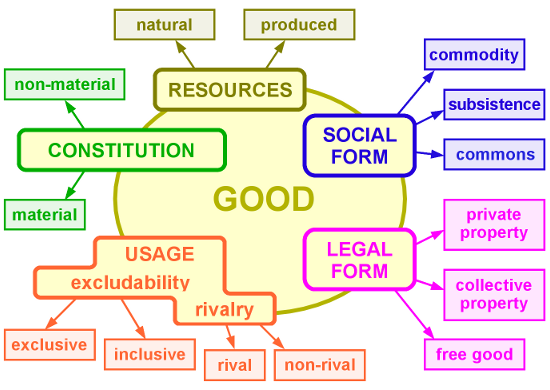
\includegraphics[width=.9\linewidth]{taxonomy-of-goods.png}
	\caption{Taxonomía de bienes o recursos.}
	\todo[inline]{¿Es necesario que el diagrama aparezca en inglés?}
	\label{fig:taxres}
\end{figure}

Volvamos a los factores de producción (tierra, capital y trabajo). El capitalismo necesita disponer de cada uno de ellos de forma que permitan producir más valor para generar más dinero y reproducir el ciclo de acumulación. Ahora bien, para que esto ocurra, necesitamos algo que muchas personas llaman contrato social pero que nosotras preferimos llamar \enquote{reglas del juego}.\revquotes{} Llamemos Estado a la entidad encargada de hacer valer las reglas del juego capitalista a través de las instituciones y de una maquinaria que garantice derechos de propiedad. El Estado proporciona lo que podríamos llamar \emph{aparato de captura} de los factores de producción para el ciclo económico del capitalismo.

Este aparato de captura se compone de tres subjetividades principales: el propietario (que posee la tierra), el banquero (que dispone del capital) y el patrón (que explota el excedente del trabajo). Estas personas (en su mayoría hombres, agentes directos de la estructura social patriarcal del ciudadano) son las cómplices humanas del parásito capitalista y se encargan de perpetuar su existencia garantizando la base material de la producción capitalista. Es decir, son los principales agentes vivos del capital y de su existencia depende estructuralmente la supervivencia del algoritmo. Hemos sido particularmente atentas en explicar estas cuestiones porque entre diferentes posiciones de izquierda (desde marxistas hasta anarquistas, pasando por feministas radicales y ecologistas) resulta extremadamente complicado distinguir al Estado del capitalismo o del mercado, y no podemos pensar en crear una fuerza política que produzca transformaciones radicales sin que entendamos de qué manera se implican estos sujetos en la configuración del estado actual de las cosas.

Hay una dimensión psicosexual de la producción además de sus componentes materiales, a través del deseo. Todas las mercancías son un poco fetiches y actúan como mediadores sociales entre las personas. Las mercancías reflejan lo que las produjo: trabajo y deseo. La relación entre el parásito (capitalismo) y el Estado es simbiótica y no parasitaria. El Imperio es la forma que toma el Estado cuando el parásito muta de la fábrica al algoritmo. El parásito requiere al Estado para garantizar los derechos de propiedad de sus propios agentes.\footnote{(añadir de conspiradores y cómplices).} Estos sujetos son los traficantes de medios de producción y configuran el aparato de captura del Estado (lo que en una configuración urbana serían los muros o en una cárcel las cadenas). La forma algorítmica del parásito, a diferencia de siglos pasados, no reprime ni suprime más el deseo sino que lo recodifica y se deposita en él. Sin embargo, la mutación del capitalismo produce fluctuaciones en el mercado, creando ciclos económicos donde el parásito es más fuerte pero también donde toca fonda antes de volver a mutar.

\begin{figure}[htbp]
	\centering
	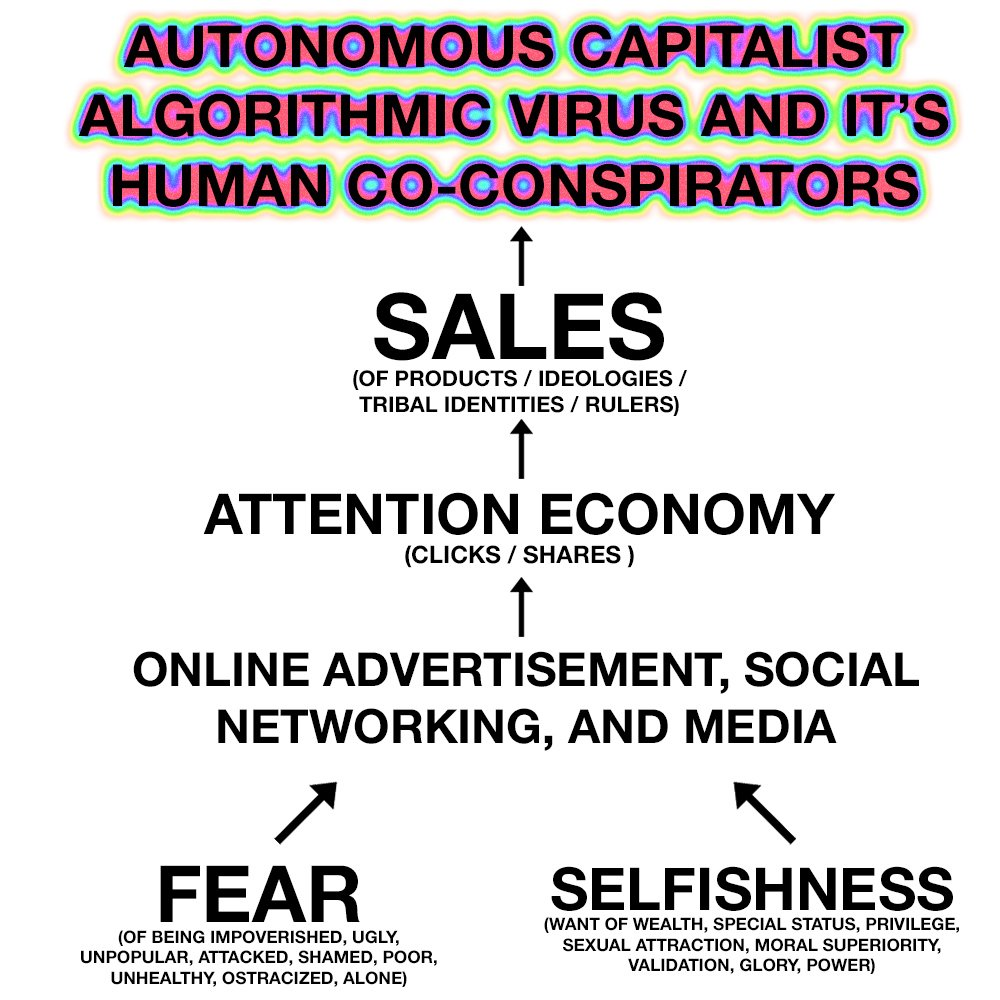
\includegraphics[width=.9\linewidth]{algorithm-capitalism.png}
	\caption[El algoritmo virulento del capitalismo.]{El algoritmo virulento del capitalismo y sus conspiradores humanos.}
	\label{fig:algoritmo}
	\todo[inline]{Valdría la pena rehacer este esquema en español.}
\end{figure}

El parásito infecta a las personas a través de mercancías que producen interacciones sociales a través del intercambio. La persona asalariada, trabajadora, accede a intercambiar su fuerza de trabajo física, intelectual, sexual o la que sea, por la potencia abstracta del dinero y éste por un objeto valorado socialmente que transforma la abstracción del dinero en reputación o prestigio, con el trasfondo del miedo a ser rechazada, a estar fuera del \emph{socius} si una no reproduce la transacción constantemente. De ese modo es que el capitalismo produce subjetividades a partir de la explotación de las trabajadoras, que en realidad no tienen una conexión real con lo que producen. En todo el planeta, aunque a diferentes escalas, esta forma de organización social produce al Gobierno y a sus súbditos: subjetividades caracterizadas por la fórmula \emph{ciudadano soldado consumidor espectador}.

No hay posibilidad de una ciudadanía tal y como se concibe hoy en día al concepto dentro de los Estados liberales democráticos. La subjetividad del ciudadano (soldado, consumidor y espectador) presupone condiciones de clase, etnia y género muy particulares que básicamente se reduce al Señor blanco, heterosexual y cisgénero, que posee propiedades, es patrón de alguien y tiene acceso al crédito y a instrumentos más complejos en el sistema financiero. Además de que esta subjetividad plantea una relación con el cuerpo propio que niega su propia castración,\footnote{Toda mercancía, en la medida en que produce al sujeto como un objeto del valor de cambio de la mercancía, también produce entre sujetos una relación de objetificación. Esta forma alienada, instrumental, de comprender a la otra persona se reproduce en su comprensión de \enquote{lo real}. Es decir, que también produce una idea sobre la naturaleza. De ahí que el capitalismo no produzca otra cosa que hostilidad y desgaste, espacios inhóspitos, pues no concibe al mundo como otro sino como instrumento.} hace creer a la forma de vida que las otras personas son lienzos donde se dibujan sus fantasías frente a otras subjetividades pauperizadas que, entre todas, están construidas para satisfacer los deseos del Señor (¡sí, del Señor feudal, de tu papá y del señor patrón, y del señor de la casa y del Señor que reina en los Cielos, la palabra \emph{Señor} tiene toda esa semántica en tu cabeza!). Entender la realidad de ese modo, y en consecuencia, la Naturaleza (y a Dios, y a la Ciencia, y al progreso), solo reafirma el poder del Estado capitalista. Por ello, cualquier movimiento político que pugne por "corregir al Estado" cuando este es la falla misma, terminará por infectar de deseos señoriales a las formas de vida que resisten a la subordinación del Espíritu que la sociedad moderna produce.\footnote{Aquí, la apuesta del populismo de Ernesto Laclau y Chantal Mouffe se posiciona por la resignificación de estos conceptos en el \enquote{sentido común}.} He ahí la complejidad de la práctica del cambio real.

\section{Más allá del Estado moderno: el Imperio}
\label{sec:imperio}

Desde un punto de vista estratégico, la transformación del Estado moderno tras la consolidación del proyecto imperialista, es el Imperio. Esta forma se caracteriza por una pulverización del poder y un cambio en los modos de producción, donde se privilegian los procesos industriales pulverizados, sin fábricas ni obreros reunidos en un mismo espacio. El Imperio se caracteriza por el auge de entidades más allá de los Estados nación, como las empresas trasnacionales, que compran representantes políticos para legislar en favor de sus intereses. Aunado a lo anterior, la policía y la publicidad, mecanismos del Estado moderno, se transforman en el Biopoder y el Espectáculo.

El Biopoder consiste en el traslado del orden de La Ley a la regulación a través de normas sin sujeto, interiorizadas. Mientras, el Espectáculo consiste en la apropiación capitalista de la imagen para mercantilizar el deseo. Estos procesos maquínicos, que definen al Imperio como fase posterior al desarrollo e implosión de los Estados-nación, tiene distintos modos de regulación, que constituyen y dan forma a su aparato de captura:

\begin{description}
	\item[Aparato socio-ideológico:] familia, tradición, religión, nacionalidad, etc. Codifica el deseo y la colonización psicológica del sujeto, establece hegemonía además de producir y mantener el estado actual de las cosas.

	\item[Aparato productivo-comercial:] finanzas, bancos, empresas corporativas, propietarios, etc. Comercialización de la producción, mercantilización del deseo para ligarlo al proceso de producción, monopolización del mercado, el valor de los desvíos que vuelve a los ricos a través de la parasitación de la mano de obra.

	\item[Aparato marcial-carcelario:] los militares, la policía, la inteligencia, el sistema de prisiones. Mantiene el estado actual de las cosas a la fuerza, la disciplina y el control de los sujetos, protege los intereses de los propietarios capitalistas y del Estado, sus fronteras, extrae recursos de otras regiones a través de la fuerza, redirige la riqueza para expandir el brazo militar del Estado e incentiva su investigación y desarrollo.

	\item[Aparato subversivo-periférico:] subjetividades colonizadas, grupos minoritarios, organizaciones criminales, la banda en sombra (\emph{shadow banking}), los mercados negros, etc. Muerte social y necropolítica. Establece la identidad de los ciudadanos mediante la otredad como diferenciación de subjetividades marginales, da un camino al lucro más allá del aparato comercial productivo.

	\item[Aparato legal de la soberanía:] el Estado, el sistema de justicia, los gobiernos, etc. Colonización el espacio geofísico, establecimiento del territorio y determinación de estratos y jerarquías sociales.
\end{description}

\begin{figure}[htbp]
	\centering
	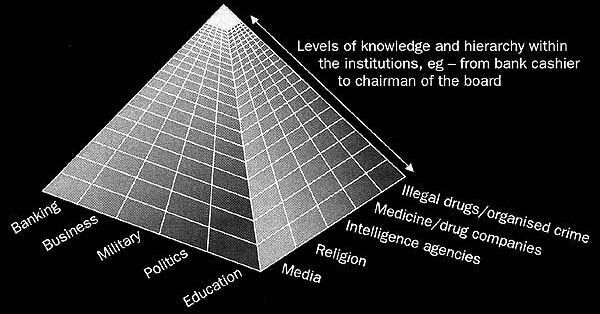
\includegraphics[width=.9\linewidth]{hierarchy-piramid.png}
	\caption{Taxonomía de bienes o recursos.}
	\label{fig:piramide}
\end{figure}

Si le damos una pensada más profunda y concreta, descubriremos que detrás de cada uno de estos dispositivos existen entidades económicas con transacciones y reglas del juego que regulan la vida social en diferentes esferas pero a dos escalas, una micro (corporal, que corresponde al Biopoder y el Espectáculo) y macro (burocrática, de legislación e infraestructura tecnológica). En principio, podríamos hablar de las cinco grandes empresas que condicionan el desarrollo de las telecomunicaciones: Amazon, Apple, Google, Microsoft y Facebook. Estas son la base material por donde fluyen información y códigos sociales, representaciones del mundo, que son reproducidas en los dispositivos personales para provocar una reacción, un deseo. Esta nueva forma del capital explota reacciones, capitaliza el placer que puede cuantificar en \emph{clicks} y \emph{shares}.

Este ciclo se basa en un delicado circuito de excitación, frustración y excitación que regula los hábitos de consumo. Se trata del modelo ideal de empresa neoliberal, un paradigma del negocio pos-industrial. La pornografía es un régimen estético que produce significados y un modo de presentación de las cosas que resulta adictivo, que permite obtener satisfacción del placer masturbatorio sobre la representación de cualquier fantasía posible materializada en videos.\footnote{De cierto modo, que el capitalismo se presente actualmente en su mayor apogeo a través de la industria farmacopornográfica (régimen toxicológico y semiótico-técnico), reproduce una concepción de la subjetividad como no castrable, cuyo horizonte parece ser el de autómatas dependientes del \emph{soma} de Huxley, personas discapacitadas, incapaces de habitar, de subsistir autónomamente.} En los foros de internet para varones adictos a la pornografía existe un nombre para el circuito pornográfico que tiene atados a tantos hombres a una forma particular de desear. Se conoce como: \emph{Porn, Masturbation, Orgasm (PMO)}.\footnote{Reddit. \emph{Don't lie to yourself\ldots P-M-O (PORN\ldots masturbation and orgasm) IS THE PROBLEM. Masturbation is just the symptom.} Disponible en \url{bit.ly/2HuEoem}.} El malestar de estos hombres cada vez más incapaces de vivir y en simbiosis con las comodidades del capitalismo que extienden el poder de sus formas tristes de vivir a otras esferas sociales, son el síntoma de este nuevo rostro de la economía. La excitación, la erección, la eyaculación, el placer y el sentimiento de autocomplacencia y control omnipotente se vuelven materias primas del proceso productivo.

\begin{figure}[htbp]
	\centering
	
\includegraphics[width=.9\linewidth]{nofap.png}
	\caption[Movimiento noFap.]{Movimiento noFap para hombres adictos a la pornografía y a la masturbación.}
	\label{fig:noFap}
\end{figure}

Por esta razón, P. Preciado señala que la pornografía es el rostro desenmascarado de la industria de la cultura y propone el concepto de \emph{farmacopornografía} para referirse al gobierno biomolecular y semiótico-técnico de la subjetividad sexual. Hay, de hecho, empresas que se encargan de regular la producción de contenidos excitantes que funcionan como mercancías con estudios explotadores y personas trabajadoras sexuales explotadas. La explotación mercantil del sexo es paradigmática porque un solo video puede producir millones de orgasmos,\footnote{Vale la pena revisar las estadísticas del tráfico de pornografía en internet. Por ejemplo, la información que libera \href{www.pornhub.com/insights/category/stats}{PornHub}.} lo que contrasta con la industria farmacéutica, donde el desarrollo de un medicamento cuesta muchísimo pero es fácilmente reproducible una vez que se obtiene y patenta una fórmula.

\begin{figure}[htbp]
	\centering
	
\includegraphics[width=\linewidth]{pillAd1.png}
	\caption{Anuncio de la píldora anticonceptiva.}
	\label{fig:anticonceptiva}
\end{figure}

\begin{figure}[htbp]
	\centering
	
\includegraphics[width=\linewidth]{pillAd2.jpg}
	\caption{Anuncio del viagra.}
	\label{fig:viagra}
\end{figure}

Así, las grandes entidades económicas capitalizan problemas clásicos de la economía como las asimetrías de información, el problema de agencia o los dilemas de acción colectiva. Además, condicionan nuestros deseos imprimiendo en nuestras psiques imágenes de lo deseable, además de crear una erística que nos enseña que esos estímulos que aprendemos a desear los podemos obtener a través de la moneda, de intercambios mercantiles. Estas empresas aprenden a través de costosas investigaciones sobre el comportamiento humano, para reproducir la servidumbre en los contenidos a través de segmentos de mercado donde se puede insertar el discurso del parásito capitalista bajo distintas situaciones y formas sexuales. PornHub es el paradigma de la industria cultural por su capacidad para producir orgasmos, para \emph{gestionar el género, la excitación, la frustración y el placer}. De este modelo de empresa se pueden extender otras versiones \emph{soft} (o blandas) que operan en otros aparatos sociales. Disney como el dispositivo que reproduce el imaginario de la jerarquía social a través de sus mitos de princesas, reyes y monstruos; MacDonalds y Coca Cola para reproducir la \hlfix{chatarrofagia}{Resaltar en cursivas.}.\footnote{Es decir, la enfermedad de la impotencia, del cuerpo enfermo, pauperizado, envenenado por las bombas mediáticas que producen la comida rápida o chatarra como lo deseable, como el lugar a donde gastar el salario. Se trata de un régimen alimenticio de productos vacíos, compuestos de harinas, grasas, azúcares y otras sustancias que funcionan bajo el mismo principio de estimulación-malestar y que producen serios daños al cuerpo a largo plazo. El paradigma mercantil de la comida en tiempos del Imperio.}

\begin{figure}[htbp]
	\centering
	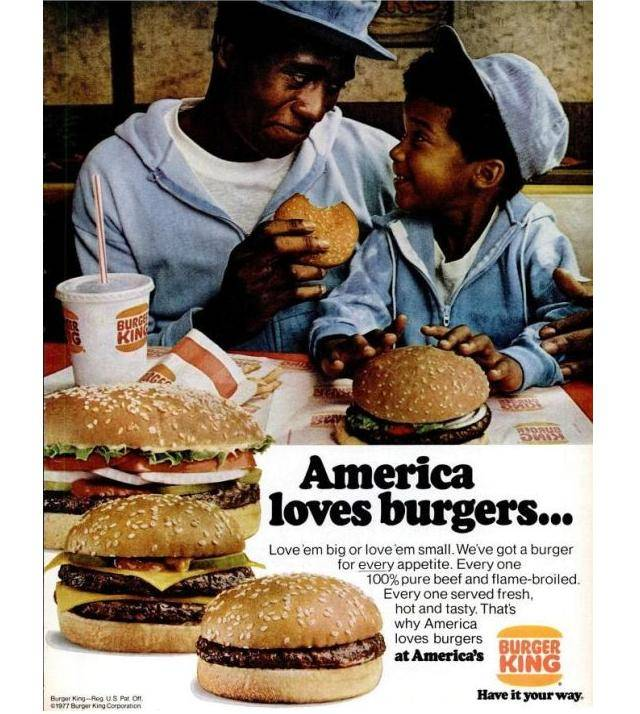
\includegraphics[width=\linewidth]{burguers.jpg}
	\caption{¡América ama las hamburguesas!.}
	\label{fig:burger}
\end{figure}

\section{La vida como trabajo y la producción de subjetividad}
\label{sec:subjetividad}

Un punto importante para comprender la transformación del Estado-nación al Imperio se encuentra en el papel del trabajo. Por ello, en este apartado analizaremos las condiciones de producción del trabajo del hombre-masa en la era cibernética. Para comenzar, tenemos que recordar que la dominación mercantil tiende a expandir sus dominios a toda área de la vida y al hacerlo vuelve trabajo a cualquier acción sujeta de la explotación. Este proceso está relacionado con la transformación de la subjetividad. No por nada el concepto central de las revoluciones de los siglos XIX y XX es la masa, una subjetividad que experimenta la realidad de la misma manera, a través del \emph{consumo estandarizado}. En este proceso, las vivencias en su forma de experiencias cognitivas dan sentido y estructura a la imaginación, es decir a la máquina deseante que es cada singularidad. Así se configura una idea del pasado (a través de Hollywood que nos enseña a desear melancólica o espectacularmente) y del futuro (el apocalipsis como una finalidad de la historia implícita en las narrativas culturales a través del tecnocapitalismo, donde la explotación se extiende a cada rincón del planeta, deja a su paso desolación y muerte para después reconstruir la \enquote{sociedad}\revquotes{}) a través de los medios que producen para las grandes audiencias.\footnote{Que dan forma a la cultura popular y al espectador televisivo en un circuito que lo posiciona como ente pasivo sentado en un sillón consumiendo comida chatarra.}

En términos concretos, la masa es el resultado de un proceso sintético en el que el individuo afronta una situación externa a él, participa en la situación y proyecta la situación en otros individuos que habitan el mismo espacio. Como ejemplo está Disney, que transmite efectivamente el deseo de casta a través de sus figuras de princesas, reyes y caballeros. Para profundizar sobre estos puntos conviene revisar los documentales de Adam Curtis, particularmente recomendamos \emph{The Century of the Self} y \emph{Hypernormalisation}.

\begin{figure}[htbp]
	\centering
	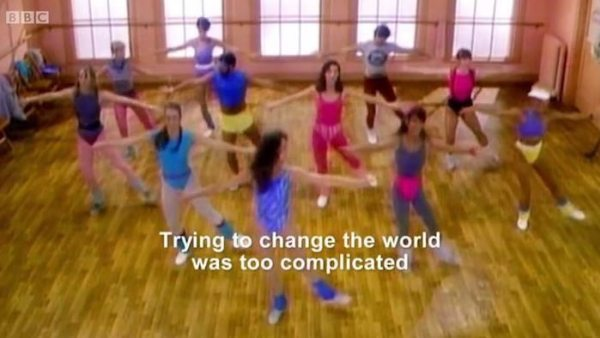
\includegraphics[width=.9\linewidth]{complicated.jpg}
	\caption[\emph{Hypernormalisation}]{Toma de \emph{Hypernormalisation}.}
	\label{fig:hypernormalisation}
\end{figure}

Nosotras hemos intentado perfilar a la subjetividad ideal del Estado moderno como algo parecido al \emph{ciudadano soldado consumidor espectador.} Solo basta recordar que el antecedente histórico del ciudadano han sido los súbditos, los fieles. Quizá desde ahí se perfila el proceso donde las multitudes devienen siempre masa a través de los aparatos de captura. El lenguaje cotidiano es muy útil para hacernos ver cómo se transmite la deuda en la subjetividad de ciudadano soldado consumidor espectador:

\begin{quote}
	paga tus impuestos\\ 
	sirve a la patria\\
	no te pierdas el descuento\ldots{}\\ 
	ni el siguiente show (la siguiente película).
\end{quote}

En esta fórmula todas las personas deben. El deber y la deuda provienen del mismo sentir (y de la misma locución latina \emph{debere}). Sin embargo, la deuda tiene una condición que ha sido entregada antes del nacimiento, como una suerte de fruto por el que hay que pagar con el pecado original durante el resto de nuestras vidas. El ciudadano \emph{debe} pagar sus impuestos, el soldado \emph{debe} honrar a la Patria, el consumidor \emph{debe} comprar y el espectador \emph{debe} mirar.

\section{Hoy en día, el capitalismo se comporta como un virus}
\label{sec:viruscapitalista}

El algoritmo del virus capitalista y el condicionamiento de desarrollo de las tecnologías mediáticas para el excedente configuran lo que se espera de las personas individualmente a gran escala. Si bien los Estados-nación dieron forma a las revoluciones burguesas fue en parte por la capacidad de leer la prensa escrita como criterio de consumo literario común suficiente para dar forma a una identidad colectiva, a una identidad de clase. Después, la radio y el cine también configuraron el potencial revolucionario de las comunicaciones. Por ejemplo, el radio creó un espacio informacional nuevo (urbanismo y psicogeografía). Esto nos muestra cómo una forma mediática representa poder y nos revela el papel clave de los \emph{medios}. Lo hace configurando el espacio a través de flujos de comunicación. La configuración de estas redes de comunicación es un catalizador para el cambio social (tabla~\ref{tab:Aristas} página~\pageref{tab:Aristas}).

En la actualidad, los modelos de masa donde un grupo recibe una sola transmisión son reemplazados por modelos donde el individuo recibe una transmisión única gracias a algoritmos reactivos que alteran la secuencia del contenido de las redes sociales y de ese modo individualiza y hace única la experiencia de consumo de cultura. La subjetividad ya no es producida como individuos en serie sino a través de segmentos.

El cambio de paradigma de modelos de gobernanza en masa a modelos en red obedece al desarrollo cibernético del algoritmo. Las sociedades disciplinarias y de control son demasiado complejas para gestionar, por lo que es más fácil fijar protocolos para gestionar redes de manera más eficiente. El espacio masivo está condicionado al número de participantes en un espacio y un momento particulares mientras que el espacio de redes se extiende y contrae en el espacio-tiempo de acuerdo a las órdenes y necesidades de la red. Es decir, su uso del capital es más eficiente porque se ajusta a las necesidades de cada momento.

Hasta ahora, este capítulo ha sido fuertemente influenciado por textos apócrifos de \#altwoke. Una idea discutida por la wikiPartida (una instancia de la Partida compuesta por gente de Wikipolítica) a partir de lo expuesto es que los modelos de gobernanza en red pueden desarrollar y expandir una cultura a través de \emph{labels}, donde los participantes son suscriptores de esta. Esto para hacer frente al problema de cómo se desplegaría una identidad FLOS que transmita cierta disposición práctica en los logos de organizaciones que la adopten. Por otro lado, nos surgen preguntas referentes a la cuestión de los medios como:

\begin{itemize}
	\item ¿qué ocurre con los gobiernos coloniales con el consumo de medios si hay masas y segmentos conviviendo y entrecruzándose? Nos referimos a medios como Netflix, Spotify y plataformas en línea además de Disney, DirecTv, Warner o, en el caso de México, Televisa.
	\item ¿Cómo se configura el imaginario de las personas en México entre Facebook, Twitter, Instagram o YouTube por un lado y Televisa, como el monopolio de sentido durante el siglo XX por el otro? Sin mencionar a Bimbo, Walmart, Coca Cola y otros grandes leviatanes. 
\end{itemize}

\section{Alternativas económicas para el futuro}
\label{sec:altfutur}

\begin{figure}[htbp]
	\centering
	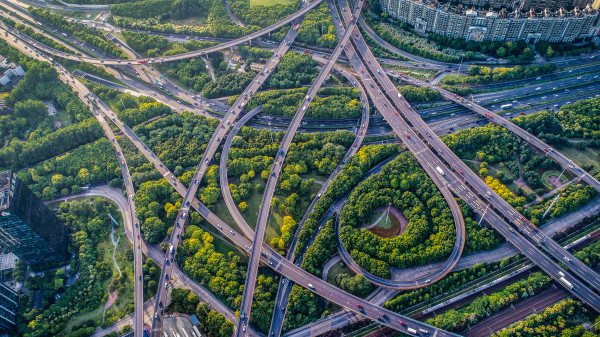
\includegraphics[width=.9\linewidth]{roads.jpg}
	\caption[\emph{Hypernormalisation}]{Toma de \emph{Hypernormalisation}.}
	\label{fig:hypernormalisation2}
\end{figure}

Hemos visto que en el entramado de complejas tecnologías que dan forma al presente, resulta extremadamente difícil accionar sin reproducir la lógica de la sociedad mercantil. El Estado, los mercados y el capital producen en conjunto una sociedad unida por un acuerdo económico donde la ética tiene un papel tan nulo que debe ser enunciada a través de imperativos morales universales porque nadie cree en ella. Y esto porque la sociedad es, en realidad, un arreglo para dar vida a las mercancías. No hay nada vivo ahí. Tiqqun acertó en señalar que la antítesis del comunismo no es el capitalismo sino la economía, y que lo que es necesario derrumbar es la dominación mercantil, que se asume como realidad última de todas las formas de vida y de todas las cosas. Para concebir acciones efectivas y críticas, tenemos que considerar que nuestras prácticas deben rebasar las estructuras formales e informales que reproducen al parásito capitalista. Para ello es de gran utilidad asumir una visión interseccional centrada en la \emph{interacción entre violencias estructurales (género, raza\footnote{Hemos utilizado la palabra raza para referirnos al discurso de raza, una ideología biologicista que sirve a los patriarcas blancos para justificar la opresión a grupos étnicos o a cualquier forma de vida no-blanca.} y clase), dispositivos sociales, el aparato de captura del Estado, la cadena de producción del capitalismo contemporáneo y el algoritmo del virus capitalista}. Esto en un contexto de complejidad donde la producción económica es comprendida en buena medida como informática, como flujos de datos con potencial de explotación. La visión de la economía neoclásica, que al informatizar la economía, le da forma de cibernética, también puede ser una herramienta de sabotaje si pensamos en los problemas de acción colectiva que necesitamos resolver para combatir la dominación mercantil como problemas de información. Algunos ejemplos que pueden ser analizados bajo esta óptica son:

\begin{description}
	\item[Gobierno representativo:] entender a los representantes como traficantes de información sobre los incentivos de sus representados (lo que en economía se conoce como \enquote{problema de agencia}\revquotes{} o \enquote{problema de agente-principal}\revquotes{}).

	\item[Burocracia:] cualquier burócrata sabe que una parte importante de la función del gobierno es el procesamiento de certificados y documentos. Una alternativa es pensar que la burocracia sea reemplazada por programadoras que mantengan un modelo de gobernanza como una máquina de información en FLOS.

	\item[Cambio climático:] un sistema de gobernanza efectivo tiene que permitirnos reconocer los costos reales y las externalidades de la producción para administrarlas en un equilibrio de Pareto.
\end{description}

Además de eso, tenemos que plantear una lógica económica para producir redes de economía solidaria que a su vez produzcan otras economías del deseo. Es decir, tenemos que combatir desde el aspecto de la infraestructura y superestructura que dan vida a la sociedad, mientras que generamos otras plataformas para producciones autónomas de deseo. Tanto la lucha por un nuevo poder constituyente como la de prácticas de destitución del Estado capitalista encuentran un entrecruzamiento en las tecnologías que condicionan su desarrollo. En ese sentido, la disciplina que se ocupa por comprender, visibilizar y transformar las relaciones de poder y sus condiciones de posibilidad[\textsuperscript{20}] en este momento histórico bien puede ser nombrada \emph{tecnocrítica}.

\begin{figure}[htbp]
	\centering
	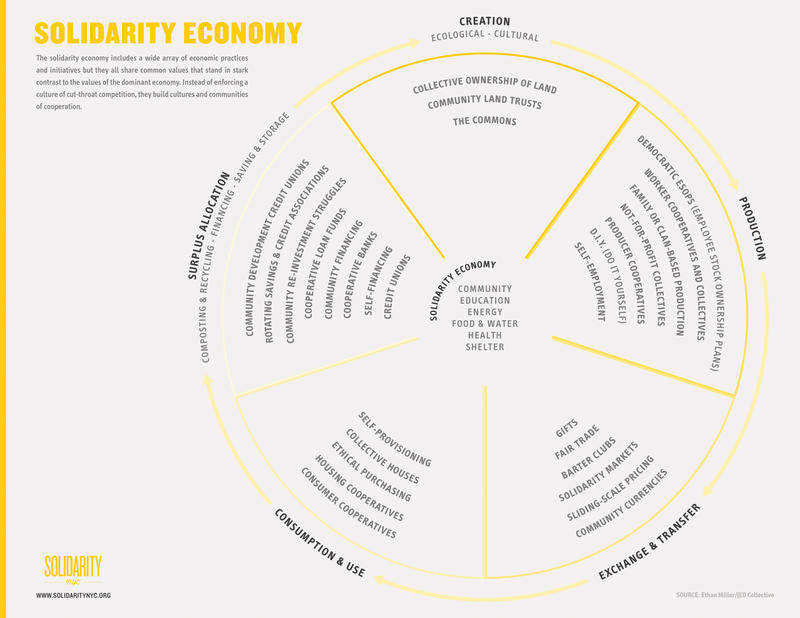
\includegraphics[width=.9\linewidth]{solidarity-economy.jpg}
	\caption{Economía solidaria.}
	\label{fig:solidarieco}
\end{figure}

Una economía tecnocrítica debería basarse en cadenas de producción que sean cíclicas y ecológicas, además de proponer trabajos orientados a la economía de la regeneración para generar empleos que restauren el medio ambiente.

\begin{figure}[htbp]
	\centering
	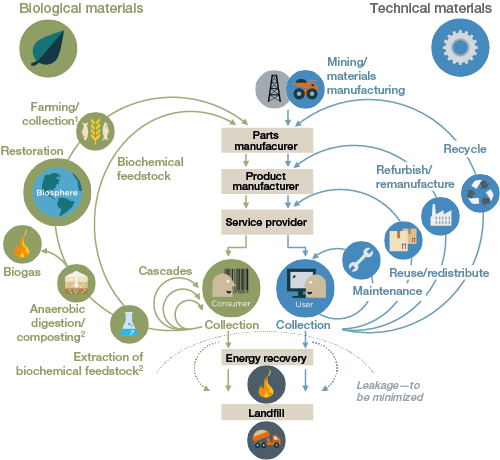
\includegraphics[width=.9\linewidth]{circular-economy.png}
	\caption{Economía circular.}
	\label{fig:circuleco}
\end{figure}

Frente a la falta de fundamentos teóricos de muchas propuestas políticas contemporáneas, nosotras creemos que el mundo donde caben muchos mundos se nutre de \emph{una ecosofía (un saber desde la Tierra), xenofeminista (que entiende las formas de opresión como el género, la raza o la clase social como tecnologías) e interseccional (que considera que distintas violencias se intersectan en las subjetividades)}. Es a partir de esta posición que tiene sentido para nosotras pensar una consideración estratégica sobre la práctica política. Hay que ir más allá de las adherencias identitarias a una facción política. Por ejemplo, la dialéctica entre horizontalismo y verticalidad es un falso dilema, ambas formas conviven en todas las relaciones grupales. Más allá de una nomenclatura en particular, nuestra posición siempre es tecnopolítica y busca prácticas anticapitalistas y antiestatales, creando comunes que permitan la gobernanza de grupos que pueden reapropiarse el valor del globalismo, descentralización, sociocracia, etc, entendiendo las subjetividades más allá del control administrativo central de la sociedad, es decir, de las normas que configuran los vínculos sociales.

La economía del don es parte de la visión de los comunes. Existen ejemplos como Grameen Bank que contribuyeron a terminar con la situación de pobreza de muchas personas en la India. Pese a que reproduce en cierto grado la lógica que las produce, sí logran generar un cambio de alto impacto. Es decir, escalable. Se trata de hacer modelos para descubrir, por ejemplo, cuántas vidas puede salvar tu proyecto, qué tan capaz es de visibilizar y crear alternativas a las violencias estructurales que sufre una persona, y encontrar proyectos clave que reduzcan transversalmente distintas formas de violencia al mismo tiempo, algo parecido al principio de Pareto.

El punto central de este apartado es señalar que la imaginación política presupone ciertas formas de hackeo a los dispositivos que dan fuerza a todo el embrujo mercantil, que son las formas abstractas de valor. El arte y el dinero tienen una relación importante en cuya génesis se pueden explorar algunas posibilidades de emancipación. La meta es reducir la dominación mercantil en estructuras económicas productivas.

\begin{figure}[htbp]
	\centering
	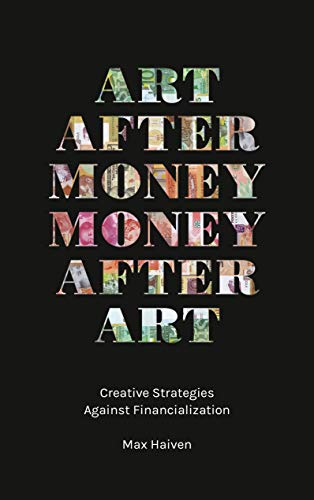
\includegraphics[width=0.6	\linewidth]{artAfterMoney.jpg}
	\caption[Recomendamos el texto de Max Haiven.]{Recomendamos el texto de nuestro colega Max Haiven.}
	\label{fig:Haiven}
\end{figure}